\documentclass{abstract_hutech}

\usepackage{cite}
\usepackage{graphicx}
\usepackage{tabularx, booktabs}
\usepackage{subfig}
\usepackage{algorithm}
\usepackage{algorithmic}
\hyphenation{op-tical net-works semi-conduc-tor}

\newcommand{\Comment}[1]{}

\begin{document}
\thispagestyle{firstpage}
\twocolumn[
\begin{@twocolumnfalse}
\vspace*{20pt}
\begin{flushleft}
\fontsize{20}{0}\selectfont{\textbf{Performance Analysis of CNN Frameworks\\
 for GPUs}}
\vspace{32pt}\par
\fontsize{10}{12}\selectfont{\textbf{In this paper, we analyze the GPU performance characteristics of five popular deep learning frameworks: Caffe, CNTK, TensorFlow, Theano, and Torch in the perspective of a representative CNN model, AlexNet. Based on the characteristics obtained, we suggest possible optimization methods to increase the efficiency of CNN models built by the frameworks. We also show the GPU performance characteristics of different convolution algorithms each of which uses one of GEMM, direct convolution, FFT, and the Winograd method. We also suggest criteria to choose convolution algorithms for GPUs and methods to build efficient CNN models on GPUs. We also analyze the scalability of the CNN models built by the deep learning frameworks in the multi-GPU context and their overhead. The result indicates that we can increase the speed of training the AlexNet model up to 2X by just changing options provided by the frameworks. }}
\end{flushleft}
\vspace{20pt}
\end{@twocolumnfalse}
]

\renewcommand{\baselinestretch}{.95} 
\section{Introduction}
Deep neural networks (DNNs) have been very successful in various machine learning tasks, such as visual recognition\cite{krizhevsky2012imagenet,vgg,RCNN}, speech recognition\cite{speech}, and machine translation\cite{machinetranslation}. Among others, the convolutional neural network (CNN) proposed by LeCun \textit{et al.}\cite{726791} is one of the earliest successful DNN models that were used to classify images. A larger and deeper CNN with more parameters usually results in a better accuracy. Thus, GPUs' massively parallel processing power makes CNNs to be trained efficiently. However, while the efficiency of a CNN on a single GPU has been improved a lot, its efficiency on multiple GPUs still shows poor scalability\cite{DBLP:journals/corr/YadanATR13}. 

In this paper, we analyze the performance characteristics of CNN models built with different deep learning frameworks and libraries. We choose five most popular deep learning frameworks, Caffe\cite{jia2014caffe}, CNTK\cite{cntk}, TensorFlow\cite{tensorflow2015-whitepaper}, Theano\cite{DBLP:journals/corr/Al-RfouAAa16}, and Torch\cite{torch}. We choose a representative CNN model, AlexNet\cite{krizhevsky2012imagenet}, to compare the five frameworks and to obtain performance characteristics.  Our comparative study provides useful insights to both end users and developers of a DNN framework. We identify which part of the GPU implementation of a framework is the performance bottleneck. This provides the developers with optimization possibilities. This will also help end users to choose a proper framework for their CNN models. 




\begin{figure}[htbp]
  \centering
  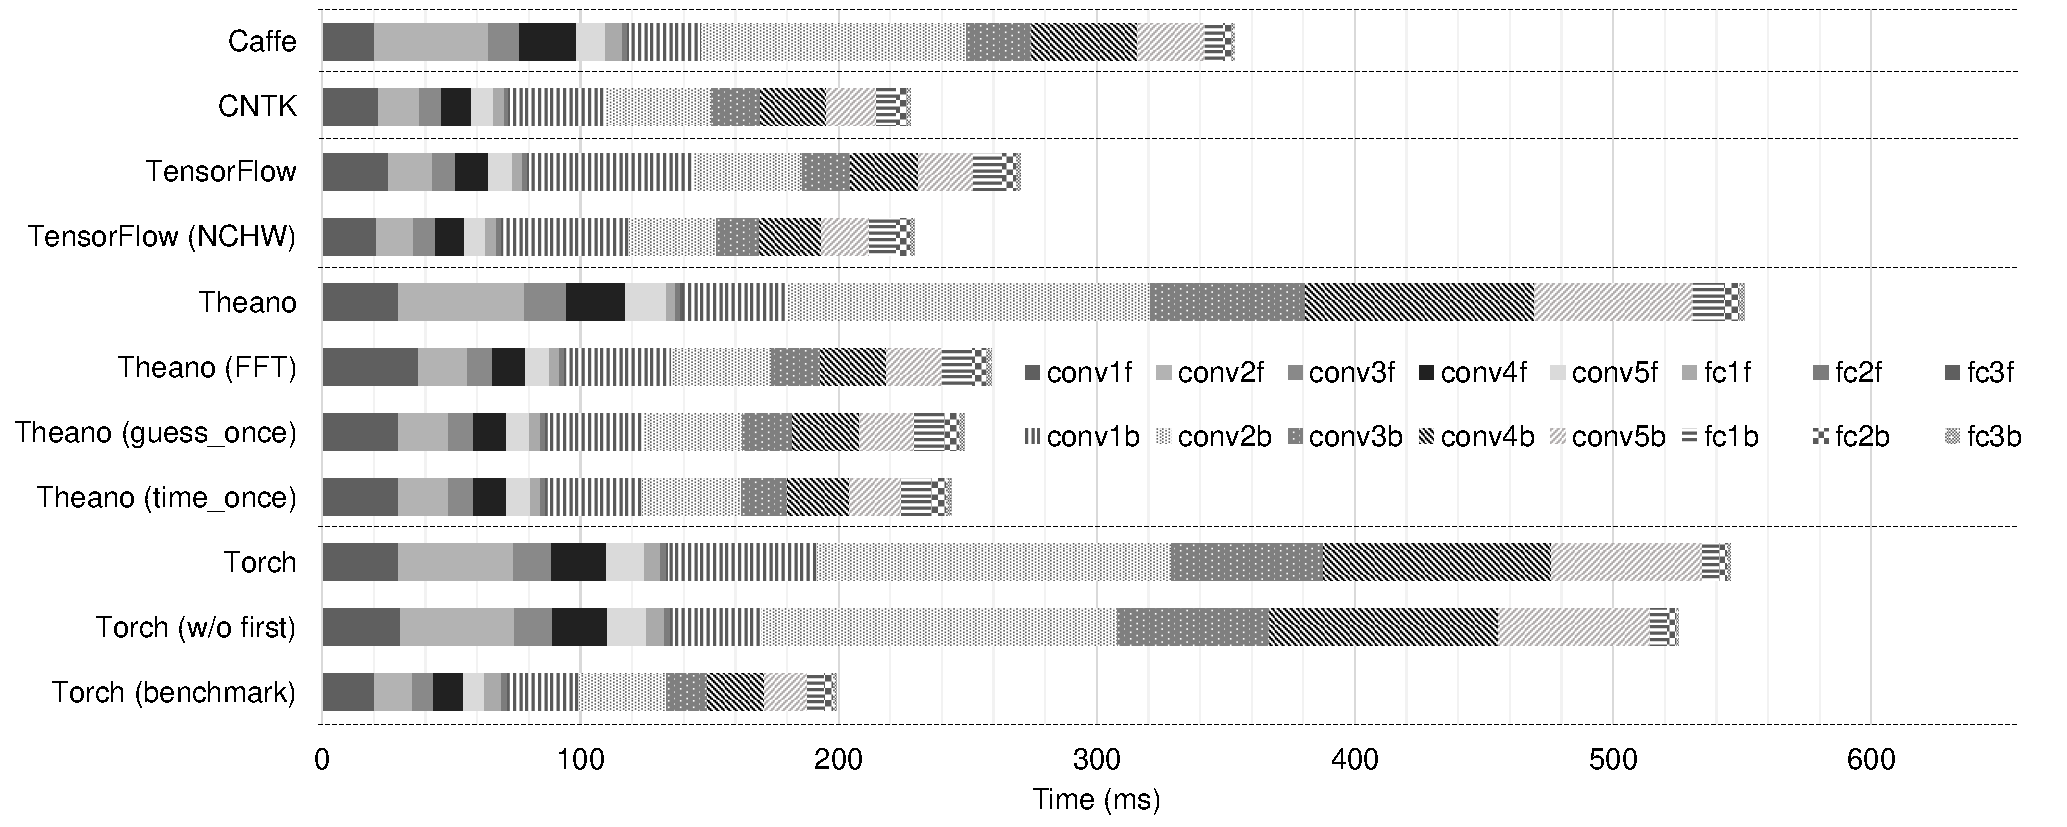
\includegraphics[width=\linewidth]{./figures/time_frameworks}
  \caption{%
The execution time of training AlexNet with a batch of imput images for differnt deep learning frameworks. 
\label{fig_time_frameworks}
  }
\end{figure}

%A = Caffe, B = TensorFlow, C = TensorFlow (NCHW tensor), D = Theano, E = Theano (FFT), F = Theano (guess\_once), G = Theano (time\_once), H = Torch, I = Torch (no backward propagation in the first layer), J = Torch (FFT), K = Torch (benchmarking) 

\section{Charactrization on a Single GPU}
\label{sec:singlGPU}
In this section, we characterize the five deep learning frameworks on a single GPU. The measurement of the layer-wise execution time of the AlexNet model for each framework is shown in Figure~\ref{fig_time_frameworks}. We observe that slight changes in framework options result in large performance differences. Options for convolution algorithm choices, data layout, and disabling useless backpropagation are most influential. We can increase the speed of training a CNN model up to 2X by just changing framework options. We do not need to modify the source code of the framework at all. 

%그 외 사소한 것으로 텐서에 네트워크 입력을 feed_dict로 주면 CPU 복사가 일어나서 매우 느리므로 FixedLengthRecordReader 등으로 주는게 좋다.
%https://github.com/tensorflow/tensorflow/issues/2919

%https://github.com/BVLC/caffe/blob/rc3/src/caffe/layers/cudnn_conv_layer.cpp#L113
%https://github.com/tensorflow/tensorflow/blob/v0.10.0rc0/tensorflow/core/kernels/conv_ops.cc#L460
%https://github.com/tensorflow/tensorflow/blob/v0.10.0rc0/tensorflow/stream_executor/cuda/cuda_dnn.cc#L933
%https://github.com/Theano/Theano/blob/rel-0.8.2/theano/sandbox/cuda/dnn.py#L285
%https://github.com/Theano/Theano/blob/rel-0.8.2/theano/sandbox/cuda/dnn_fwd.c#L227
%https://github.com/soumith/cudnn.torch/blob/R5/SpatialConvolution.lua#L166




\section{Characterization of Convolution Algorithms}

In this section, we compare the performance of different convolution algorithms on a single GPU. The total training time of \textsf{FFT} is the best for all batch sizes. However, for $3 \times 3$ convolution kernels with a small batch size, \textsf{Winograd} performs better than \textsf{FFT} while \textsf{FFT} scales better with a large batch size. 

\begin{figure}[htbp]
  \centering
  \subfloat[The execution time on each layer] {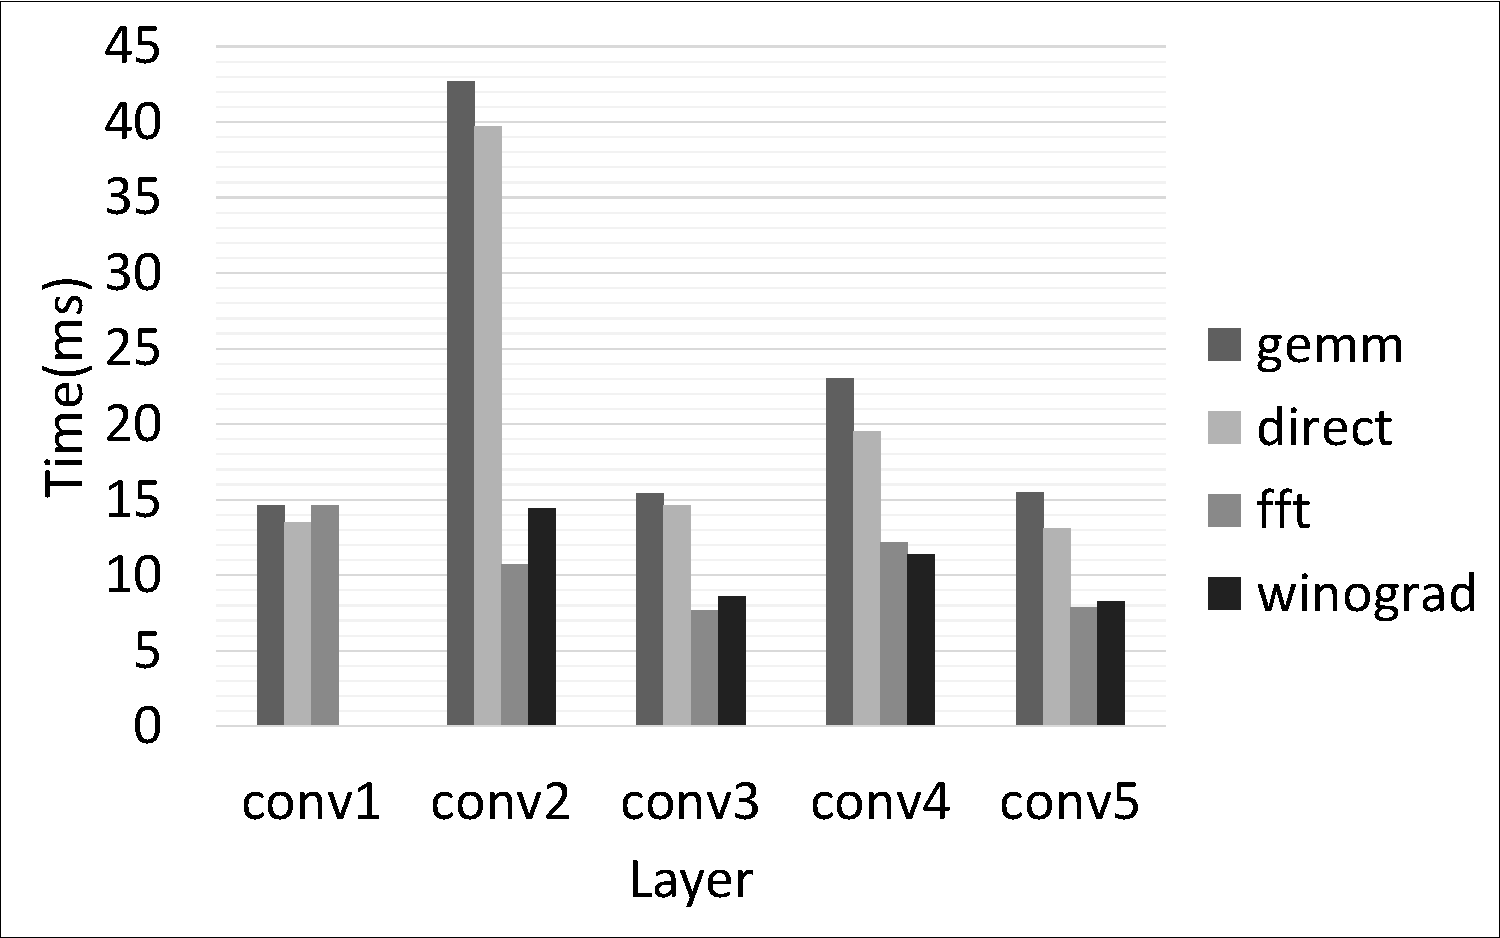
\includegraphics[width=.8\linewidth]{./figures/layerwise_fwd}
  \label{fig_layerwise_fwd}}

  \subfloat[The execution time by batch sizes] {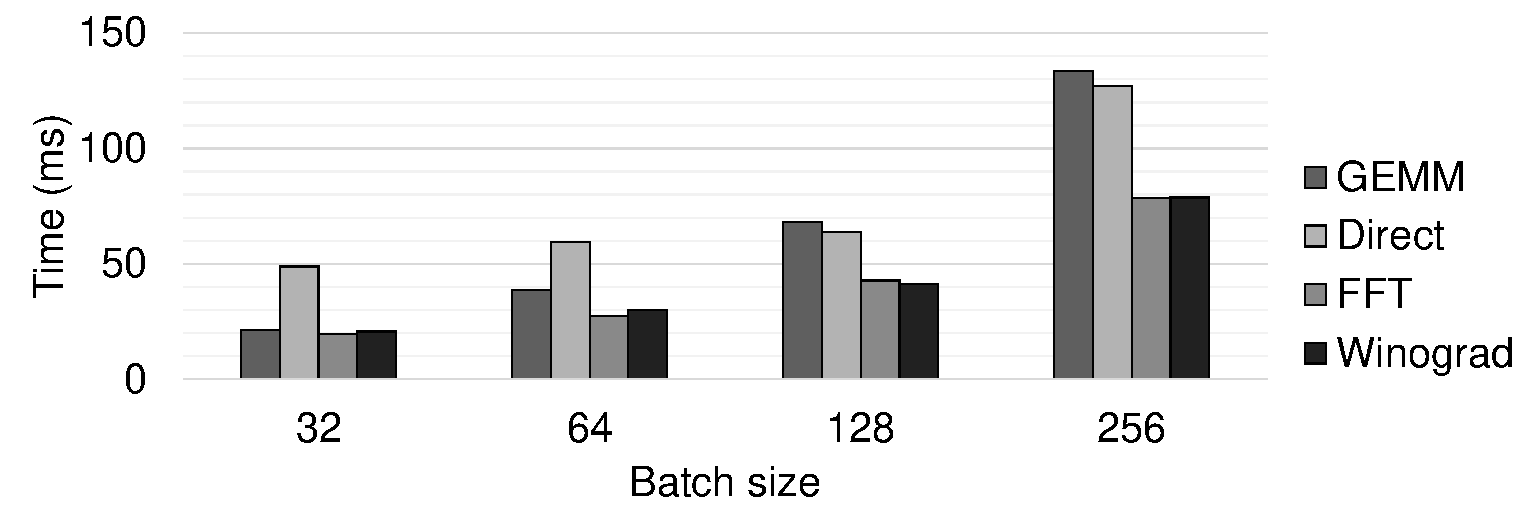
\includegraphics[width=.8\linewidth]{./figures/gpu_time_fwd}
  \label{fig_gpu_time_fwd}}


  \caption{The execution time of the forward computation.}
  \label{fig_layerwise}
\end{figure}

\begin{figure*}[htbp]
  \centering
  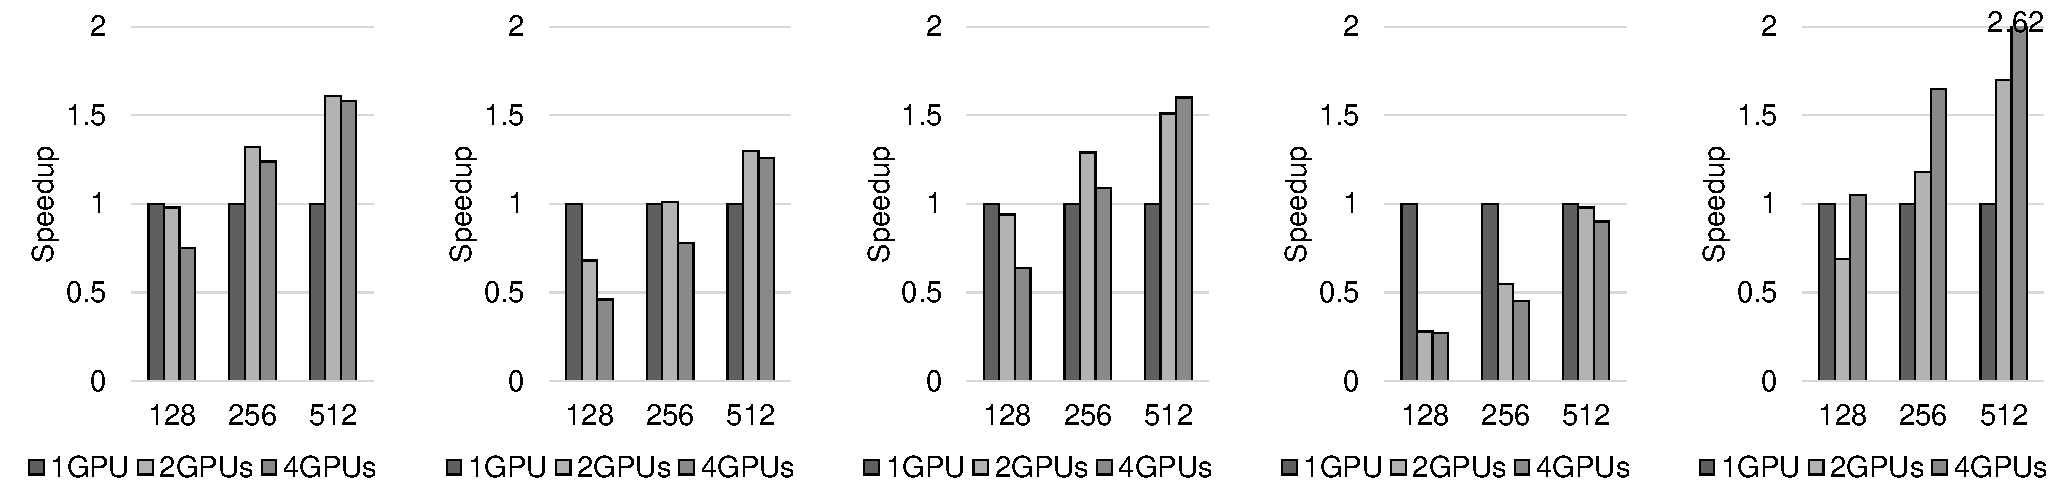
\includegraphics[width=.8\linewidth]{./figures/MG}
  \subfloat[Caffe]{\makebox[.19\linewidth][]{}}
  \subfloat[Torch]{\makebox[.19\linewidth][]{}}
  \subfloat[TensorFlow]{\makebox[.18\linewidth][]{}}
  \subfloat[CNTK]{\makebox[.18\linewidth][]{}}
  \subfloat[CNTK 1bit-SGD]{\makebox[.18\linewidth][]{}}
\caption{Speedup (over a single GPU) of multi-GPU training of the AlexNet models.}
\label{fig_mg}
\end{figure*}

 The result tells us that \textsf{FFT} is usually the fastest because of much less FP operation count (\textit{i.e.}, much less algorithm complexity). Especially, \textsf{FFT} is much faster than others in \textsf{conv2} with $5 \times 5$ convolution filter because the complexity of \textsf{FFT} does not depend on the filter size. \textsf{Winograd} also reduces FP operation count by more than a half. Thus, its performance is comparable to \textsf{FFT} in the layers with $3 \times 3$ convolution filters (\textsf{conv3}, \textsf{conv4}, and \textsf{conv5}).
\section{Multi-GPU Support}
\label{multi-GPU}
In this section, we characterize the performance of the AlexNet models on multiple GPUs. The AlexNet models are trained on one, two, and four GPUs. Ideally, the training time of AlexNet is expected to be reduced to $\frac{1}{N}$ when $N$ GPUs are used. However, this is not true because of the data transfer caused by the gradient data exchange. Figure~\ref{fig_mg} shows the speedup obtained by multi-GPU training of our AlexNet models with different batch sizes and numbers of GPUs. We see that a bigger batch size makes the speedup higher. We also see that the scalability of each framework is quite poor. 

TensorFlow-like data transfer and computation overlapping will be helpful to improve the performance. Reducing the size of gradients by approximating the exact value with less accuracy (\textit{e.g.}, using the half-precision FP format or only 1-bit like CNTK) will also improve scalability a lot. Reducing the number of gradients by resizing and pruning the CNN model will also work.

\section{Conclusions}


%\section*{Acknowledgment}

%The authors would like to thank...

\bibliographystyle{humantech}
\bibliography{ispass17}
%\nocite{*}

\end{document}
